\subsection{Glissando-Effekt}\label{subsec:Glissando_Effekt}
Auch für den Glissando-Effekt war es notwendig einen Test durchzuführen, um die Genauigkeit der Töne festzustellen. Wir verwendeten auch hier anstatt unseres PCB einen Funktionsgenerator. Um die Frequenz einzustellen, wurde das Tool \textit{SignalTap Logic Analyzer} in Quartus eingesetzt um auf das Register der Frequenzmessung mit den Messresultaten zuzugreifen. Schlussendlich wurde der Ton mit der App \textit{Tonal Energy Tuner} auf dessen Genauigkeit gemessen. Die App gibt diese Genauigkeit direkt in Cent an. Die Messung umfasst alle Frequenzen aus der Tabelle \ref{tab:Toene_Frequenzen} in Kapitel \ref{subsec:Musiktheorie}. In Abbildung \ref{img:Validierung_Glissando} sind alle diese Abweichungen aufgezeigt. Die blaue Kurve  zeigt die Resultate, wenn die Frequenz kleiner eingestellt wurde als der anzunähernde Ton. Die orange Kurve zeigt die Resultate, wenn die Frequenz grösser eingestellt wurde als der anzunähernde Ton. Wie zu sehen ist, ist auch diese Funktion genauer als \SI{8}{Cent}. Interessanterweise nimmt bei beiden Einstellungen offenbar die angenäherte Frequenz mit höheren Tönen immer mehr ab. Da die Frequenzmessung wie zuvor besprochen mit grösseren Frequenzen immer mehr Abweichung hat, ist dies auch erklärbar.\\
Weshalb die Kurve nicht wie in der Frequenzmessung immer positiv wird, erklärt die Abbildung \ref{img:Erklaerung_Glissando}. Da bei tiefen Frequenzen die gemessene Frequenz eher tiefer ist als die wirkliche, bedeutet dies, dass der IST-Wert grösser ist als der Messungs-Wert. Der Glissando-Effekt nähert nun die Differenz zwischen dem gemessenen Wert und dem SOLL-Wert an. Dies bedeutet, dass der angenäherte Wert immer noch die Abweichung zwischen IST und Messung hat. Bei den hohen Frequenzen ist es genau umgekehrt. Die Messung ist nun höher im Vergleich zum IST-Wert. Somit bewirkt der Glissando-Effekt in diesem Szenario, dass die angenäherte Frequenz kleiner ist als der SOLL-Wert.


\begin{figure}[h!]
	\centering
	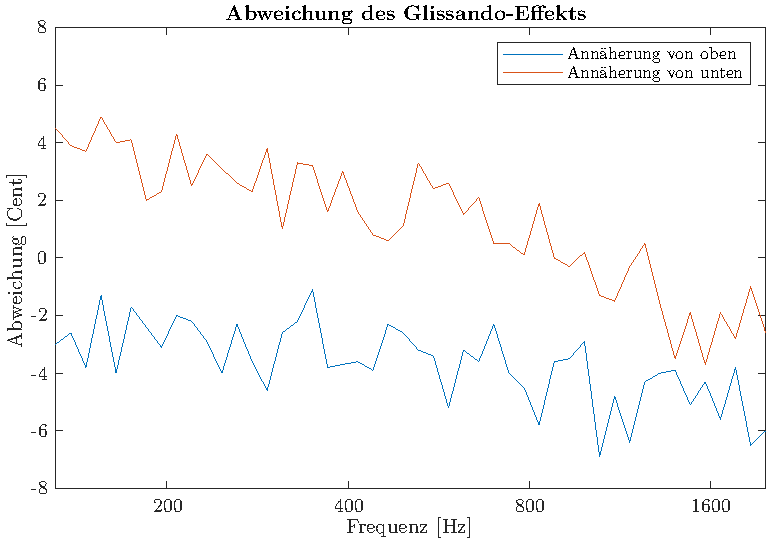
\includegraphics[width=0.9\textwidth]{Validierung_Glissando.pdf}
	\caption{Resultate der Validierung des Glissando-Effekts} 
	\label{img:Validierung_Glissando}
\end{figure}  

\begin{figure}[h!]
	\centering
	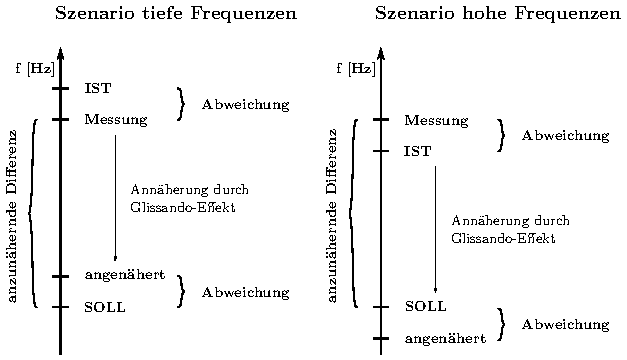
\includegraphics[width=0.9\textwidth]{Erklaerung_Glissando.pdf}
	\caption{Erklärung der beobachteten Änderungen} 
	\label{img:Erklaerung_Glissando}
\end{figure} 

\begin{table}[H]
	\centering
	\caption{verwendete Messmittel}
	\label{tab:Glissando_Messmittel}
	\begin{tabular}{l|l|l}
		\textbf{Messmittel} & \textbf{Bezeichnung} \\
		\hline\hline
		Funktionsgenerator & MSZ-M-0051   \\ \hline
		SignalTap Logic Analyzer & -    \\ \hline
		Tonal Energy Tuner App &  -   \\ \hline
		
	\end{tabular}
\end{table}

